\section{Vocabulario de Accidentes de Bicicletas}

Para el vocabulario asociado con los accidentes de bicicletas se han tomado como referencia los datos proporcionados por el ayuntamiento de Madrid.  \cite{datosMadrid_accidentesDeBicicleta}. En estos datasets se muestran los accidentes de tráfico con implicación de bicicletas dentro de la jurisdicción del ayuntamiento.
\newline
Se han añadido además algunos datos no proporcionados en estos datasets, como es el Municipio, el id de la vía u otros, ya que se han considerado necesarios para la definición de un vocabulario reutilizable y aplicable a otros datasets.
\newline
Este vocabulario se ha definido con el objetivo de ser válido tanto para accidentes de tráfico de bicicletas como de automóviles u otros vehículos. Aun habiendo partido de un dataset en el que se representaban los accidentes relativos al primer caso, todos los elementos definidos pueden ser utilizados en cualquier tipo de accidente. Debido a que este trabajo está enfocado a crear una aplicación para la seguridad de bicicletas, se ha partido de esta base, pero podría ser perfectamente reutilizado para otro tipo de accidente añadiéndole propiedades necesarias para los mismos como podrían ser la velocidad, el numero de pasajeros...
\newline
La organización del conjunto de datos se hará siguiendo el diagrama \ref{fig:diagramaOntologAccid}

\begin{figure}[h]
	\centering
	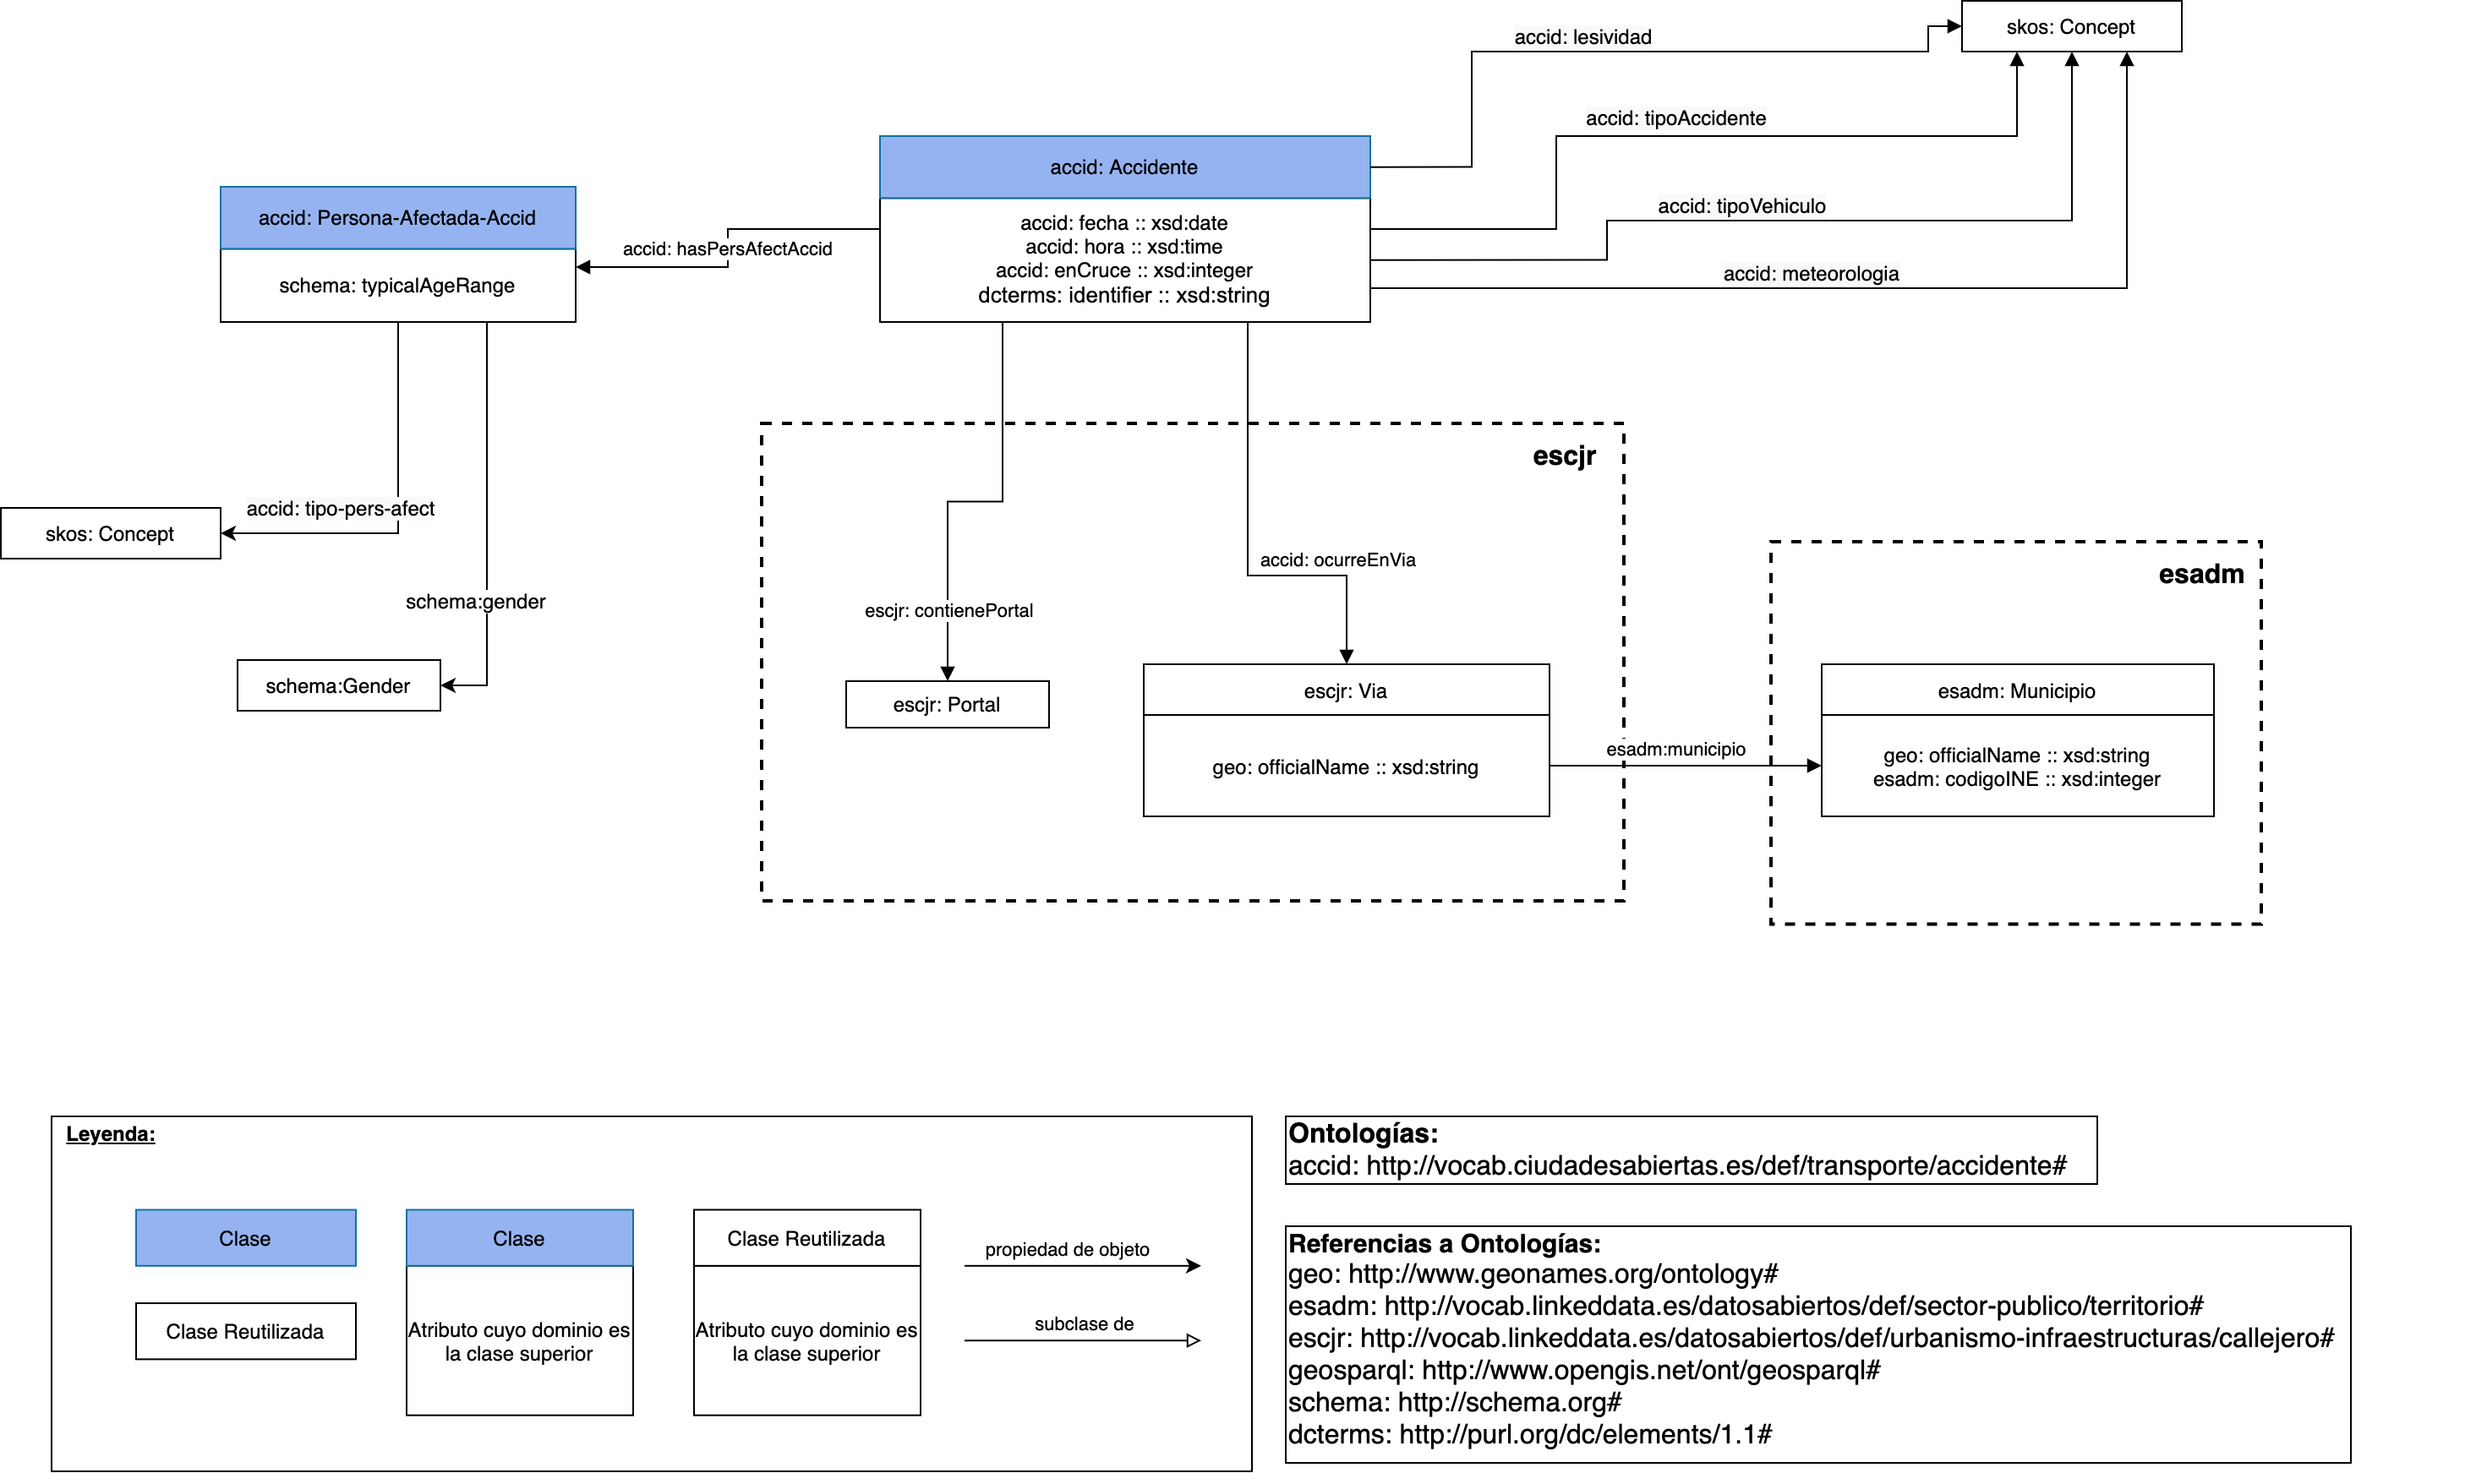
\includegraphics[angle=0, width=1\textwidth]{images/diagramaAccidBici.png}  
	
	\caption{Diagrama de Ontología de Accidentes.}
	\label{fig:diagramaOntologAccid}
\end{figure}


Para la representación de los datos de accidentes de trafico se han definido varias clases y propiedades. Se han reutilizado elementos ya definidos en el vocabulario de Callejero \cite{ciudadesbiertas_callejero}, de Territorio \cite{datoabiertos_municipio} y de Schema \cite{schema_org}.

\clearpage
En la siguiente tabla se muestran los Namespaces usados.

\begin{figure}[h]
	\centering
		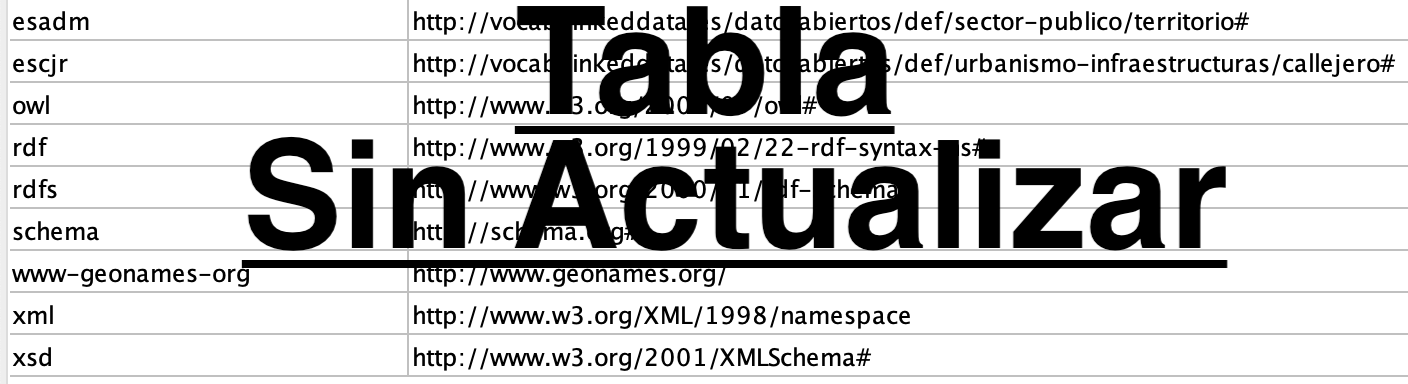
\includegraphics[angle=0, width=0.8\textwidth]{images/tablaIRIsAccidentesBici.png}  
	\caption{Namespaces usados para Accidentes}
\end{figure}




Se ha optado por mantener la separación de elementos como fecha y hora, calle y numero debido a que en la fuente de origen están así dispuestos y en la posterior aplicación final que se va a construir será más conveniente tener esa información por separado, para poder disponer de datos a horas con menos luminosidad o calles completas(sin conocer la posición exacta), por ejemplo.


Para este conjunto de datos se ha optado por añadir, además de los ya proporcionados por la fuente de origen del ayuntamiento, nueva información como la propiedad ``esCruce``, el municipio, el tipo de vía o el identificador de vía. Son propiedades inferidas de la información proporcionada que permiten que sea más sencillo su tratamiento y uso, para esta u otras aplicaciones que puedan tener estos datos.
EsCruce se obtendrá del nombre de la calle, del cual atendiendo a varios patrones se puede determinar si el accidente ha ocurrido en una intersección de dos o más vías.
El Municipio se ha añadido para su posible reutilización posterior utilizando otros datasets de otras localidades, para este caso será siempre Madrid.
El Identificador de Vía se obtendrá comparando el nombre de la vía y su tipo con el Callejero de Madrid, el cual proporcionará este valor único que represente la vía.
El tipo de vía finalmente se ha eliminado del vocabulario ya que no tiene relevancia para los datos obtenidos de éste, más allá de la obtención del identificador de vía. En cualquier caso, si fuese necesario se podría obtener a partir del nombre de la calle, aunque no se ha considerado relevante para añadirlo a la ontología.

En este conjunto de datos se ha hecho un cambio relevante con respecto al original y que será detallada en el capítulo Transformaciones en los vocabularios. Los accidentes que han ocurrido entre un cruce de vías se han separado en tantos registros como vías interfieran. De este modo será mucho más simple la búsqueda de accidentes ocurridos en una calle y se podrá hacer una búsqueda más sencilla de ellas. Se podrá identificar si dos o más registros pertenecen al mismo accidente por el número de expediente, el cual se conserva igual en ambos.

Este vocabulario ha sido propuesto para ser incluido en el repositorio opencitydata en el ISSUE \url{https://github.com/opencitydata/transporte-accidentalidad-trafico/issues/1}.




